\documentclass[11pt, a4paper]{article}

\usepackage[utf8]{inputenc}
\usepackage{fullpage}
\usepackage[parfill]{parskip} % Empty line instead of indentation
\usepackage{graphicx}
\graphicspath{ {images/} }
\usepackage{listings}
\usepackage{mathtools}
\usepackage{amssymb}
\usepackage{eurosym} %Euro symbol
%\usepackage[ngerman]{babel}
\usepackage{cancel} % Cancel fractions
\usepackage{units}
\usepackage{xcolor}
\usepackage{setspace}
\usepackage{subcaption}

% TODO replace some of these \newcommands with \DeclareMathOperators
\newcommand\braces[1]{\left(#1\right)}
\newcommand\brackets[1]{\left[#1\right]}
\renewcommand{\vec}[1]{\underline{#1}}
\newcommand{\mat}[1]{\underline{\underline{#1}}}
\newcommand{\abs}[1]{\left\lvert#1\right\rvert}
\newcommand{\norm}[1]{\left\lVert#1\right\rVert}
\newcommand\tr[1]{\mathrm{tr}\br{#1}}
\newcommand\average[1]{\left\langle#1\right\rangle}
\newcommand{\acos}[1]{\mathrm{acos}\braces{#1}}
\newcommand{\asin}[1]{\mathrm{asin}\braces{#1}}
\newcommand{\intend}[1][]{\ \mathrm{d}#1}
\newcommand{\derivative}[2][]{\ \frac{\mathrm{d}#1}{\mathrm{d}#2}} %\derivative[a]{b}
\newcommand\expectedValue[1]{\mathbb{E}\braces{#1}}
\newcommand\variance[1]{\mathbb{V}\braces{#1}}
\newcommand\setequal{\overset{!}{=}}
\newcommand{\gerquote}[1]{\glqq#1\grqq}
\DeclareMathOperator{\sign}{sign}
\definecolor{AI-BLUE}{rgb}{0,0.57,0.87}

\onehalfspacing
\setlength\parindent{0pt}
\allowdisplaybreaks

\title{TITLE}
\author{AUTHOR}
\date{\today}

\makeatletter
    \setlength\@fptop{0\p@}
\makeatother

\begin{document}
\thispagestyle{empty}

\begin{titlepage}
    \begin{center}
    \vphantom{0cm}
    \huge \textbf{Hardening artificial neural networks against specifically constructed adversarial input data} \\
    \vspace{4cm}
    %\LARGE \textbf{Report}\\
    \normalsize
    Written Master Thesis Report \\
    for the Masters Program of \textcolor{AI-BLUE}{[Applied Computer Science]}\\
    at the Ruhr-University Bochum\\
    in the Summer Term 2016\\
    \vspace{4cm}
    %\normalsize
    \textbf{Submitted by}\\
    B. Sc. Christian Andreas Mielers (108 011 204 956)\\
    \vspace{1cm}
    \today \\
    \vspace{1cm}
    \textbf{Supervisors} \\
    PD Dr. Rolf P. Würtz \\
    M. Sc. Andreas Nilkens
    \end{center}
\end{titlepage}

\newpage
\pagenumbering{arabic}
\setcounter{page}{2}

\tableofcontents

\newpage
\section{Introduction}
\label{sec:introduction}

As the problems people try to solve with the aid of computers become more and more complex, their ability to write software that can keep up with those aspirations does not follow suit. Solving more complex problems with software does not only incur the cost of finding viable solutions and formalizing them in computer code, but also the cost of integrating all the necessary components, organizing their interactions, ensuring they use common resources in a well-defined manner, and testing all of the above. These tasks grow essentially super-linearly in difficulty, and can thus quickly become harder than the problem that the system was initially meant to solve.

One way out of this dilemma that people turn to increasingly often is the usage of machine learning techniques. The goal of machine learning is to free people from the burden of finding and programming a solution. In order to do so, a \emph{model} is defined which embodies the structure of a possible solution on a highly abstract level. However, such a model as potentially a myriad of \emph{parameters}, and no knowledge of reasonable values for those parameters can be assumed. What gives machine learning its name and makes it feasible despite the many unknown parameters is the learning method. This is a method to find a working configuration of parameters based on \emph{training data}. In \emph{supervised learning}, the algorithm that performs the learning is provided numerous pairs of an exemplary input and the corresponding desired output that the model should deliver. From these pairs, it extracts, or \emph{learns}, the relationship between input and output data, and codifies it in the model's parameters. In this manner, the need for a handcrafted solution is eliminated. The downside to this approach is that learning algorithms usually require a copious amount of training data to find good parameters. However, this drawback is increasingly often offset by the reduced software complexity, since machine learning models usually have a well-defined theoretical foundation with ready-made software available.
% TODO write something about verification with test data?

% TODO substantiate claim that ANNs are among the top machine learning models
Among some of the most momentous machine learning models are \emph{artificial neural networks (ANNs)}. They are inspired by discoveries from the field of neural biology and incorporate them into models that, on a very abstract level, resemble brain structures on the detail level of individual neurons. The workings of these  neuron are greatly simplified, but in this way they can be easily connected in large bulks, empowering the resulting network to solve difficult tasks with impressive precision. ANNs are mainly used to two types of tasks: \emph{classification} and \emph{regression}. While the latter is concerned with learning a function $f: X \rightarrow Y$ that maps input data to the desired output values, it is the former that will be of interest within the scope of this thesis. Classification instead aims to assign each input to one category out of a predefined set of categories. The data used to train the network is structured accordingly: it consists of the input data and a \emph{label} that denotes its class.
% TODO note that learner for neural networks is "gradient descent"?

% TODO illustrate image classification
One area where neural networks are particularly successful is \emph{image classification}, the task of classifying an object by from a digital photo of it. A big part of the success here can be attributed to a special variant of ANNs, called \emph{Convolutional Neural Networks (CNNs)}. These networks focus on local features in the input by applying \emph{filters} in a convolution operation, thereby curtailing redundancies in the free parameters. Combined with the focus on local features, this efficient use of free parameters allows for much larger and thus more powerful networks.

% TODO illustrate training and test steps with an image
When training a neural network for an image classification task, one desires a CNN to not only classify the images used for training correctly, but to infer and learn the fundamental characteristics of each class. Only then will the network be able to \emph{generalize} its classification capabilities to the previously unseen images it will encounter in productive use. To gauge a network's ability to generalize, another data set, called the \emph{test set} is usually withheld while training the model. The experimenter can then evaluate the performance on this set outside of training, thus obtaining an estimator for field performance of the model.

In the past, ANNs in general and CNNs in particular have shown convincing results not only on training data but also test data. However, recent discoveries have indicated that the generalization capability of most neural networks is not as strong as one might guess from test set performance. While networks certainly can classify unseen input with high reliability, it is possible to find minute transformations of correctly classified test data, on which the network will predict another class with high confidence. The changes that need to be applied for this to work are miniscule and undetectable to the human eye. The resulting images are called \emph{adversarial examples (AEs)}.

In the initial publication a rather complex method for creating those images was presented. A major impediment of this method was the excessive computational power and time required to produce AEs. Fortunately, a follow-up paper greatly improved the feasibility of this process by introducing a gradient-based procedure for generating AEs. In that manner a considerable amount of AEs can be generated in a reasonable time frame, enough to allow for reasonable quantitative analysis of the AE's properties. Therefore, this thesis will look at various statistics of larger groups of AEs, including their spectra and the ways these spectra differ from those of unadulterated images. Regarding the spectra, we will also look at the distribution of values with regards to the frequency and orientation.

Furthermore, the process of generating adversarial examples can be inspected on a considerably larger scale. Plots for the network confidence on images in the process of being turned into AEs will provide insights on the process with regards to iteration count, and serve as the foundation for attempts to predict whether an image can be successfully made adversarial. Data on the success rate of converting images to adversarial examples will be presented, both per original and adversarial class as well as overall figures.

The aforementioned results will be obtained with multiple data sets and various network layouts and parameter configurations. The latter will also allow for inspection of the impact of parameter choice on various statistics.

% History
%% What is a neural network
%% Strengths
%% Industry applications
%% The problem with adversarial examples
%% What this thesis is about
% Future prospects










\newpage
\section{Artificial Neural Networks}
\label{sec:artificial-neural-networks}
In the area of machine learning, artificial neural networks are some of the most widely studied models. They stem from insights into the workings of real, biological brains in the field of neural biology. Here, the individual neuron is used as the fundamental unit of computation. A schematic version of the biological variant is shown in figure \ref{fig:biological-neuron-schematic}.

\begin{figure}[htp]
	\centering
	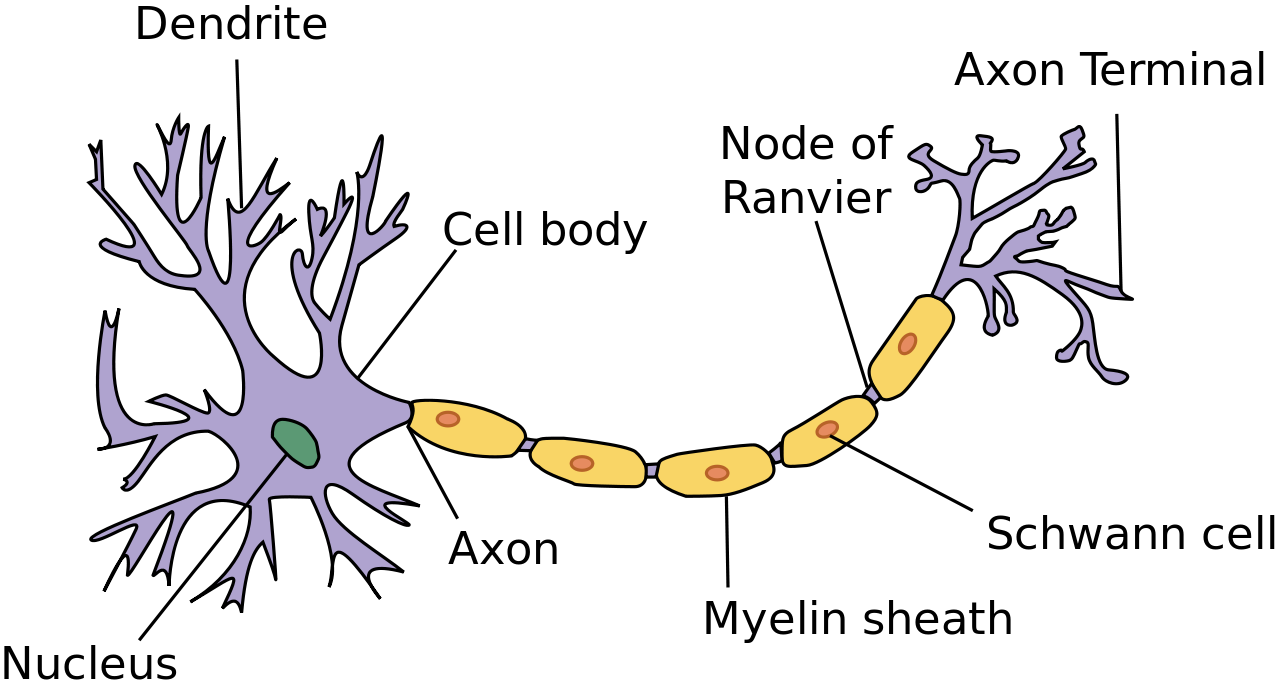
\includegraphics[width=0.5\textwidth]{images/biological_neuron.png}
	\caption{Schematic of a biological neuron, taken from \cite{biological-neuron-schematic}}
	\label{fig:biological-neuron-schematic}
\end{figure}

% TODO be a bit more precise here with the chemistry
A neuron receives incoming electrical pulses, called \emph{action potentials}, from the axons of other neurons via its dendrites. A connection between an axon and a dendrite is called a \emph{synapse}. These synapses can vary in strength, so the intensity of the received pulse is modulated by the synaptic connectivity. Multiple action potentials may arrive in the soma, the cell body of a neuron, in quick succession, causing the membrane potential of the soma to increase. If enough action potentials arrive within a short time via strong synapses, this may cause the cell in question to initiate an action potential which traverses along its axon. This can be considered to be a decision of the sell to pass the message on to other cells.

An artificial neuron as used in an ANN mimics this process, but in a greatly simplified form. All action potential rates are represented by real numbers\footnote{Floating point numbers in a computer system}. A visual representation is provided in figure \ref{fig:artificial-neuron-schematic}.


\begin{figure}[htp]
	\centering
	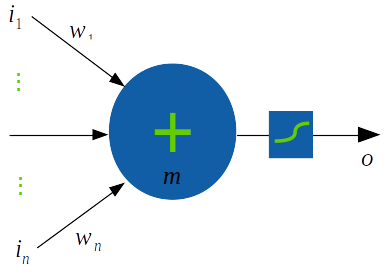
\includegraphics[width=0.45\textwidth]{images/artificial_neuron.png}
	\caption{Schematic of an artificial neuron}
	\label{fig:artificial-neuron-schematic}
\end{figure}

The first thing to note is that the input to the neuron is now formalized as a vector $\vec{i}$ with components $i_1 \dots i_n$, where $n$ represents the number of inputs that influence this neuron. Each input value $i_j$ is multiplied with a \emph{weight}, denoted by $w_j$. This weight can be thought of as an abstraction of the synaptic strength between two neurons. Then, all of these input-weight pairs are summed up to realize the counterpart to the membrane potential, labeled $m$. To form the neuron's output $o$, one last step is neccessary. In biological neurons, the rate of outgoing spikes of a neuron is not linear in the incomming spikes. Thus, a nonlinear \emph{activation function} is applied to the membrane potential $m$, symbolized by the sigmoidally shaped line in the rectangular box in figure \ref{fig:artificial-neuron-schematic}. If that activation function is called $\sigma$, the mathematical operation performed by a single neuron can be summarized according to equations \eqref{eq:neuron-math-membrane-potential} and \eqref{eq:neuron-math-activation-function}.

\begin{align}
	m &= \sum_{i=1}^n w_n \cdot i_n = \vec{w}^T \vec{i} \label{eq:neuron-math-membrane-potential} \\
	o &= \sigma \braces{m} \label{eq:neuron-math-activation-function}
\end{align}



% TODO will it only become especially important in chapter 3, or also in other places?
Take note of the fact that the very first step performed on the input is essentially an inner product. This will become important later on, especially in chapter \ref{sec:adversarial-examples}. Several activation functions are possible. A plot of 3 common choices is given in figure \ref{fig:activation-functions}.

\begin{figure}[htp]
	\centering
	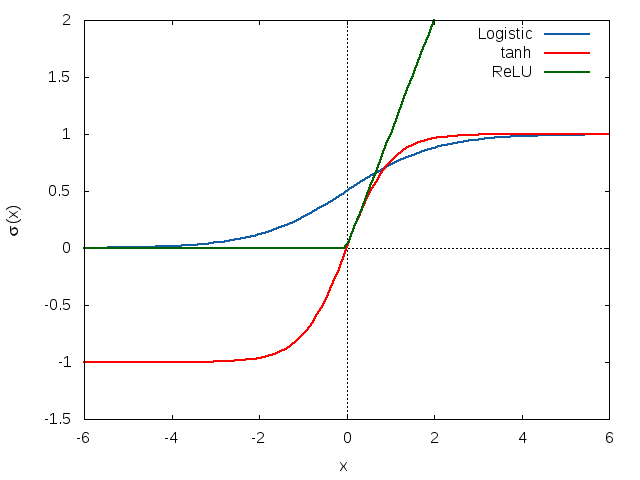
\includegraphics[width=0.6\textwidth]{images/activation_functions.png}
	\caption{Logistic sigmoidal, hyperbolic tangent and ReLU activation functions}
	\label{fig:activation-functions}
\end{figure}

Out of these, the easiest to justify is the logistic sigmoid. If the output is to represent the neuron's firing rate, it must not become negative, and it must saturate because of the refractory period required by biological cells. Under these conditions, the logistic function is a simple continuous choice. The hyperbolic tangent is a linearly transformed version of this. While its negative range may be harder to interpret biologically, the option to output negative values may relieve the trainable parameters of a network of some demand for computational power, thus facilitating training. Despite being non-continuous and having no upper bound, the ReLU is the most popular activation function according to \cite{deep-learning}. The networks utilized in this thesis mostly make use of the $\tanh$ and ReLU activation functions.

Since a single neuron as described above consists only of an inner product and a one-dimensional non-linearity, its computational power is limited. Artificial neural networks rely on thousands of neurons to perform their tasks. This gives rise to the question of how to connect all those neurons. Conceptually, one could link them up in such a way that a neuron that receives input from another neuron while at the same time delivering input to that same neuron (either directly or via proxy neurons), forming a cycle. This is sometimes done in practice and is called a \emph{Recurrent Neural Network (RNN)}, but is out of scope for this thesis. Instead, neurons will be organized in \emph{layers}, as shown in figure \ref{fig:neural-nework-structure}. %TODO

\begin{figure}[htp]
\centering
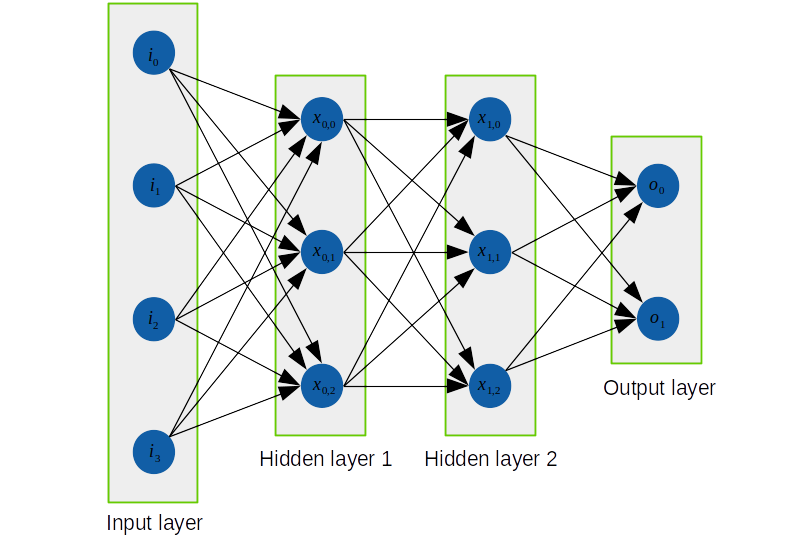
\includegraphics[width=\textwidth]{images/network_layout.png}
\caption{Structure of neuron arrangement in an ANN}
\label{fig:neural-nework-structure}
\end{figure}

% TODO back up claim that input layer is called "first and "lowest" layer
% TODO use top-down image instead of left-right. Requires to reformulate the text a bit.
Here, each layer contains numerous neurons, none of which share a connection. This means that there is no interaction within a layer and thus it seems reasonable to inspect the actions of a network in a layer-by-layer fashion. The layer on the left is often called the "first" or "lowest" layer, and it is the spot where the input data is feed into the network. Therefore, its neurons deviate from the description given in figure \ref{fig:artificial-neuron-schematic} and equations \eqref{eq:neuron-math-membrane-potential} and \eqref{eq:neuron-math-activation-function}. No computation takes place here, the data is taken as-is and used as input for the layer above.

% TODO be more specific about the universal approximation theoren
% TODO describe layers as homeomorphisms according to http://colah.github.io/posts/2014-03-NN-Manifolds-Topology/
In the figure the layer above the input contains 3 neurons and is named "Hidden layer 1". Hidden layers are those that are neither input nor output and thus do not communicate with any system outside the network. Note that each neuron here has two indices: The first one designates the layer affiliation and the second one identifies the individual neuron. The first hidden layer is followed by a second one. A neural network can conceptually have an unlimited amount of hidden layers, but at least one is necessary to satisfy the \emph{universal approximation theorem} which attests that for every function, there exists a neural network that can approximate said function to a arbitrary but fixed accuracy\footnote{However, this is of limited practical use, since the theorem makes no statement about the required number of neurons, or how to set the weights.}.

A further notational simplification can be made at this point. Equation \eqref{eq:neuron-math-membrane-potential} described the operation of a single neuron as an inner product. If we treat the output of \emph{Hidden layer 1} as a vector $\vec{x_0}$ and the output of \emph{Hidden layer 2} as another vector $\vec{x_1}$, the entire operation of the second hidden layer can be described by a matrix-vector product according to equations \eqref{eq:layer-math-membrane-potential} and \eqref{eq:layer-math-activation-function}.

\begin{align}
	\vec{m_1} &= \mat{W_{1}} \, \vec{x_0} \label{eq:layer-math-membrane-potential} \\
	\vec{o_1} &= \sigma \braces{\vec{m_1}} \label{eq:layer-math-activation-function}
\end{align}

where $\sigma \braces{\vec{m_1}}$ indicates the element-wise application of the activation function to the membrane potentials. If the weight vectors used in equation \eqref{eq:neuron-math-membrane-potential} are used as row vectors of $\mat{W_1}$, then this is an equivalent description on a higher level of abstraction. This can of course be done analogously for the other layers of the network.

Beyond biological plausibility, this formalism provides another justification for using activation functions at all. If they were not part of a neural network model, each layer would solely perform a matrix-vector product, which, due to their linear properties, could be collapsed into a single matrix-vector product, greatly reducing the model's capacity to describe complex relations between input data and output data.

% TODO source for softmax function
The last layer generates the output of the network. It too can in part be described as a matrix-vector product. It may also share the same activation function as other layers, in which case its functionality is mostly identical with hidden layers. However, this is sometimes inappropriate. In regression, for instance, the range of the function to be learned may go far into the negative range, well below $-1$. None of the activation functions shown in figure \ref{fig:activation-functions} are capable of modelling this. Similarly, in classification, it might be desirable for the output to represent the probabilities of an input belonging to each of the classes. While all of the discussed activation functions include the range $[0-1]$, thereby making such a representation possible, other activation functions specifically suited for output layers, like the \emph{softmax function}, can force those properties.

% TODO Deep dream
% TODO Akin to layered processing in vision
% TODO Back up the claim that first layer is usually feature extractor / corner detector.
The relatively recent machine learning trend going by the name of \emph{deep learning} builds extensively on this layered architecture of neural networks. Specifically, \emph{deep} neural networks use many more hidden layers than just 1, in contrast to the preceding networks, which were ex post named \emph{shallow} networks. The central hypothesis of this approach is that the various layers of a network will learn to perform distinct, hierarchically structured functions. Typically, the first layer (or first few layers) are expected to become low-level feature extractors, providing basic information for the higher layers. In vision tasks, for example, one can often observe that the lowest layer works as a corner detector, because the geometry within an image often contains the most important information. The following layers the hopefully extract features with an increasing level of abstraction, e.g. combining corners to edges and more complex shapes and contours. The last layer is tasked with making the final decision regarding the input object's class, using the presence of those high-level features as the basis for its choice.

% TODO some networks make use of this? Sure its not all of them?
% TODO glorot formula
% TODO caffe does glorot initialization slightly differently
One question that has not been addressed yet is how to actually set the weights. Under normal circumstances there is no closed form solution to compute the optimal parameters for a model. Thus, an training process that starts with a random set of weights and then iteratively improves on them is used. To accomplish random initialization, values for all weights are drawn from one of various distributions. Common choices are uniform, normal distributions. In 2010, a more sophisticated method has been proposed in \cite{glorot-understanding-deep-nn-training}. It still relies on a uniform initialization, but the limits are set for each layer individually, in order to retain the variance the data as it flows through the layers of the network. Some networks in this thesis make use of this advanced initialization.

In order to improve the thusly initialized weights, it is first necessary to define a way to quantify how well (or poorly) a given set of parameters performs. To this end, an \emph{loss function} (also called \emph{objective function} or \emph{error function}) is used, which combines the predictions of a network with the training labels to provide an estimate of its performance. In other words, it is a function that maps labeled input data and the parameters to a scalar value. A common loss function is the \emph{Mean Squared Error (MSE)} given in equation \eqref{eq:mse}, where $N$ is the number of data points and $\vec{\hat Y}$ and $\vec{Y}$ are vectors containing the prediction and true label, respectively. In multinomial classification tasks, the \emph{cross entropy} loss given in equation \eqref{eq:cross-entropy-loss} \cite{caffe-cross-entropy} is a good choice if the predictions for all classes are to be interpreted as probabilities (meaning they are required to add up to 1). Here, $\vec{\hat Y}$ is a matrix containing all predicted class probabilities for all $N$ data points and $\vec{Y}$ is a vector indicating the true class.

% TODO source for MSE
% TODO make this more readable
\begin{align}
	\text{MSE} &= \frac{1}{N} \sum_{i=1}^N \braces{\vec{\hat Y}_i - \vec{Y}_i}^2 \label{eq:mse} \\
	\text{Cross entropy} &= \frac{-1}{N} \sum_{i=1}^N \log{\braces{\mat{\hat Y}_{i, \vec{Y}_i}}} \label{eq:cross-entropy-loss}
\end{align}

% TODO possible source for gradient descent: "Stochastic Gradient Descent Learning in Neural networks"
The goal of neural network training is usually to minimize the loss function (although it could be maximization depending on the formulation of the loss function). This is most often accomplished with a \emph{stochastic gradient descent} on the loss function mentioned above w.r.t the weights of the network\footnote{In practice, the gradient w.r.t a lot of weights can be computed very efficiently by exploiting properties of the chain rule, a method known as \emph{Backpropgation}, or Backprop for short.}. A simple, one-dimensional case is given in figure \ref{fig:gradient-descent}.

% TODO reduce the borders within the image
\begin{figure}[htp]
	\centering
	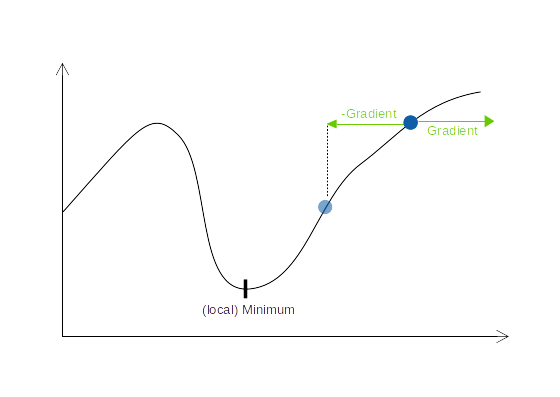
\includegraphics[width=0.7\textwidth]{images/gradient_descent.png}
	\caption{Illustration of the gradient descent method}
	\label{fig:gradient-descent}
\end{figure}

Starting at an arbitrary point, the gradient always points in the direction of steepest ascent. The idea of a gradient descent is to move the parameters (in this case the weights) into the opposite direction in order to descend the slope of the loss function. Following the left-oriented green arrow, the network with parameters corresponding to the blue dot would adopt the parameters corresponding to the transparent variant slightly to the left, resulting in a reduced loss. This process is iterated many times in order to hopefully reach a minimum that represents a good solution to the training process.

The magnitude of the gradient us usually used as an indication of how much the weights should be changed. Note that there can be many complications, for instance, if the blue dot had started to the left of the local maximum near the right side, it might have found a smaller local minimum than the one marked in figure \ref{fig:gradient-descent}.

%% Biologically inspired
%% Very popular
%% Successful
%% Neuron is a radical simplification
% Neural networks discard time
%% Some math
%% Layered
%% Activation functions
%% Error function
%% Gradient descent, Backpropagation
%% Deep learning
%% Recurrent vs. feed-forward










\subsection{Convolutional Neural Networks}
% TODO rewrite this paragraph. It sucks.
% TODO are really ALL networks in this thesis CNNs?
A special kind of ANN that has proven to be particularly effective on image data is the \emph{Convolutional Neural Network (CNN)}. All networks used in this thesis are CNNs. They differ from conventional networks in the way some of the layers function. CNNs contain \emph{convolutional layers}, which, as the name implies, perform convolutions on the incoming data. In a way, the weight matrix that connects the layer's neurons with the neurons of the previous layer is replaced with \emph{kernels} or \emph{filters}, with which the incoming data is convolved. A schematic representation of this procedure is given in figure \ref{fig:convolutional-layer}.

% TODO activation function
\begin{figure}[htp]
	\centering
	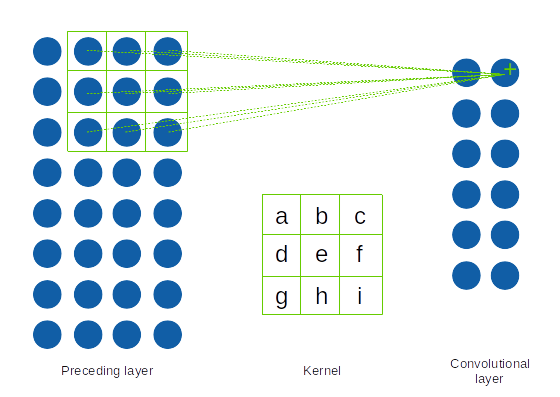
\includegraphics[width=0.8\textwidth]{images/convolution_layer.png}
	\caption{Schematic of a convolutoinal layer's functionality}
	\label{fig:convolutional-layer}
\end{figure}

The easiest way to understand this is to imagine the left part as an input image of size $4 \times 8$, with an immediately following convolutional layer. In this example, the convolutional layer has one filter of size $3 \times 3$, though other sizes are possible. Since these are 2 arrays of two-dimensional shape, the computation of the convolutional layer's output can be computed by a two-dimensional convolution, save for possible activation functions. As can be seen in figure \ref{fig:convolutional-layer}, this produces an output of size $2 \times 6$. The size reduction is a consequence of neglect to deal with the edges of the input image, the filter is only centred on those areas where the input is completely defined\footnote{While the reduction from $4 \times 8$ to $2 \times 6$ may seen extreme, it is worth mentioning that the number of pixels "lost" only grows with the \emph{circumference} of the input data, so for a more reasonably sized image, the output map will only be slightly smaller.}.

However, the figure also indicates that there is a different, connectionist perspective on this process. In this view, the neurons on the right still connect to the preceding neurons with weights and compute an inner product. There are 2 major differences to a conventional layer. First, each neuron is only connected to 9 input values, instead of all of them, leading to the first considerable reduction in the number of weights that need to be trained. Second, all neurons use \emph{the same weights} to connect to their (distinct) 9 inputs, giving rise to the term \emph{weight sharing}. This again greatly reduces the number of weights, to a constant count of 9, regardless of the size of the previous layer. For a quick comparison, a conventional layer with 12 neurons would lead $12 \cdot 32 = 384$ parameters. Additionally, in contrast to the constancy of the 9 weights in a convolutional layer, this figure would grow with the product of both layer sizes. For an image size with practical applications, this rapidly becomes impractical.

% TODO source for the claim that most information in images emerges from local features
Using a convolutional layer does not just reduce the number of parameters that require training, but also tailors the network's structure to the specific properties of image related tasks. Since each neuron in a convolutional layer is connected only to a small, contiguous region of the input image, the learning algorithm is forced to train the kernel weights in such a way that they focus on local features. Since a lot of distinctive information in images such as edges, corners and textures emerges from local features, this mechanism confers the benefit that data not relevant to those features is implicitly ignored. This shares some similarities with the concept of receptive fields human vision, which are also local.

The convolutional layers of the CNNs used in this thesis and in practice are slightly more complicated than the above explanation suggests. If a convolutional layer had only used kernel, it would only be able to extract a single feature from the input data. Because this is insufficient, convolutional layers generally have numerous kernels, each of which gets convolved with the input independently, producing multiple outputs called \emph{maps}. Concordantly, a convolutional layer is able to receive multiple maps as input. The scenario with multiple input and output maps is depicted in figure \ref{fig:convolutional-layer-maps}.

\begin{figure}[htp]
	\centering
	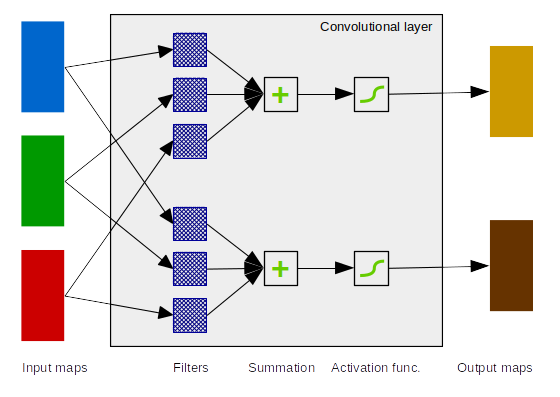
\includegraphics[scale=1.00]{images/convolution_layer_maps.png}
	\caption{Schematic of a convolutional layer with multiple input and output maps}
	\label{fig:convolutional-layer-maps}
\end{figure}

On the left side we see 3 input maps. On the lowest layer, the input maps correspond to the 3 color channels red, green and blue\footnote{When using a grayvalue image, there is only 1 channel and therefore only 1 map}. On the right side the convolutional layer produces 2 output maps. The process for computing one such output map is as follows: First of all, each input map gets convolved with a filter that is unique to that map (and to the output map. The resulting arrays are summed up to form one array of the correct shape. Depending on the network layout, processing the array element-wise with an activation function may be a part of this step. This process is performed multiple times with distinct filters, depending on how many output maps are desired. Since for every pair of an input map and an output map there is exactly one filter, the total number of filters in a convolutional layer is $M \cdot N$, where $M$ and $N$ are the counts of input and output maps, respectively.

% TODO Source for Max-Pooling
The parcimony with free parameters required by a convolutional layer to produce an output map makes it feasible to use many filters and consequently produce a great deal of output maps. This empowers the CNN with considerable modeling capacity, but also poses the challenge of dealing with all that generated output. CNNs have one more mechanism at their disposal to solve this specific problem. To reduce the dimensionality of the feature maps, they use \emph{pooling} layers, which execute subsampling on the maps as indicated by figure \ref{fig:pooling-layer}.

\begin{figure}[htp]
	\centering
	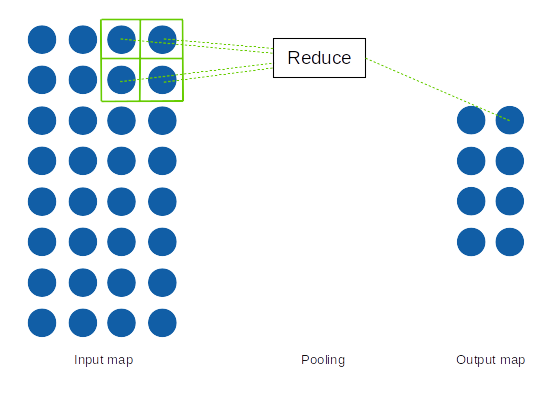
\includegraphics[scale=1.00]{images/pooling_layer.png}
	\caption{Schematic of a pooling layer downsizing an input map}
	\label{fig:pooling-layer}
\end{figure}

The input is located to the left and comprises 32 neurons arranged in a two-dimensional $4 \times 8$ array. The pooling layer condenses the information to 8 neurons in a $2 \times 4$ array. This is done by segmenting the input into regions that do not necessarily need to be disjoint or cover the entire input. Each of these segments covers a small, usually rectangular region of the input. An operation that reduces all values in a segment to a single value is then applied. All scalars from each segment together constitute the output of the pooling layer. Common reduction operations include averaging and taking the maximum. The networks in this thesis exclusively use the latter.

As one can see the amount of data has been greatly reduced. However, if pooling is applied to the output maps of a convolutional layer, it is reasonable to assume that critical information is retained. Unless the input image contains very high frequency information apart from noise, the convolutions should yield similar values at adjacent points. A max pooling operation then would simply select the best match for a given feature. Besides greatly reducing the amount of data to be handled, this method also confers the benefit that translational invariance is increased since the exact location of a specific feature is discarded by the pooling.

%Translation invariance

%% Focus on local features
%% Receptive field
%% Usefulness in image processing
%% Weight sharing -> Efficient use of free parameters
%% No edge treatment
%% More than one filter per conv layer
%% Channels and maps
%% Max-Pooling

\section{Adversarial Examples}
\label{sec:adversarial-examples}

% TODO might Neural Representation and Neural Computation be a good cite for this?
% TODO is dynamic-field-theory-movement-preparation a good cite?
% TODO cite more things, especially for the molecular modelling
In trying to recreate the learning power of the human brain on a computer, one can focus on various levels of abstraction. A system could potentially model all the chemical processes that happen within and around cells and their synapses on a molecular level. Less drastically, one could work with aggregates and averages of these values in order to retain most of the biological components and create a time-dependent system this way. Alternatively, larger groups of neurons could be used as the basic building blocks for a larger system \cite{dynamic-field-theory-movement-preparation}, operating on a level of high abstraction from chemical processes.

% TODO source for state-of-the-art claim
% TODO source for surpassing human performance
The connectionist view is based on the proposition that ANNs as described in section \ref{sec:introduction} model the functionally relevant processes in biological brains in sufficient detail. Such systems have shown state-of-the-art performance on diverse tasks, in some cases even surpassing human performance. One important property that is required of machine learning models is the ability to \emph{generalize}. If given training data and the desired labels, a neural network should not merely learn to classify this specific data\footnote{This could be solved perfectly by just storing the data and the label}, but also learn to correctly classify new and unseen data, so long as it is reasonably similar to the training data, even if the specifics vary.

% TODO illustration of training and test, e.g. flowchart
To probe a model's generalization ability, a part of the available data is usually withheld from training, effectively making it unseen data. After training, the networks performance on this set can be evaluated to obtain an estimate of its performance in practice. Even though training and test data may be a bit stronger correlated than the training data and the input in a productive environment\footnote{For instance due to changes in illumination or camera equippment}, ANNs have shown reasonable generalization ability.

% TODO source for calling under scrutiny
However, some discoveries have called this ability under scrutiny. A recent paper \cite{intriguing-properties-of-neural-networks} demonstrated that a state-of-the-art neural network can be tricked into misclassifying an input image by applying minuscule changes, even small enough to be imperceptible by humans. The thusly altered images are called \emph{adversarial examples (AEs)}. Their existance is problematic because from a generalization standpoint the minimum requirement would be that a network classifies visually indistinguishable images identically if it has a high confidence on one of them. However, network confidence is not an obstacle to finding AEs, they exist even for images where the network makes a certain and correct class affiliation assertion. Figure \ref{fig:intriguing-properties-ae} shows such an adversarial example\footnote{even though \cite{intriguing-properties-of-neural-networks} contains a link to full-resolution images, it is dysfunctional as of the time of this writing (Error 404)}.

\begin{figure}[htp]
\centering
	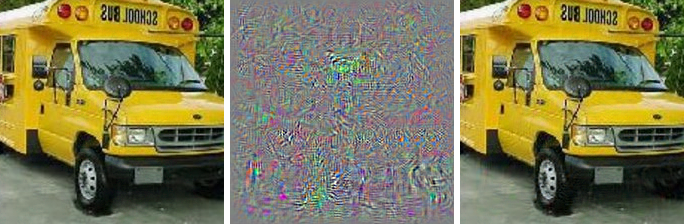
\includegraphics[width=\textwidth]{images/intruiging_properties_ae.png}
	\caption{Original image (left) and adversarial example (right, classified as \emph{ostrich, Struthio
camelus}) with magnified difference in the middle, as presented in \cite{intriguing-properties-of-neural-networks}}
	\label{fig:intriguing-properties-ae}
\end{figure}

It is apparent that the function represented by the network is undesirably discontinuous and lacking in smoothness, leading to strongly fragmented classification regions. Adversarial examples can exist as a result, they occupy regions proximal to to training points in the data manifold, but on the other side of such a discontinuity. Naturally, the question arises how to find such perturbations given a (training or test) image. In \cite{intriguing-properties-of-neural-networks}, this is posed as an optimization problem according to equations \eqref{eq:ae-formalization-minimize} - \eqref{eq:ae-formalization-valid}.

% TODO \vec and \mat
\begin{align}
	\text{Minimize $\norm{r}_2$ s.t.} \label{eq:ae-formalization-minimize} \\
	f(x + r) &= l \label{eq:ae-formalization-label} \\
	x + r &\in \brackets{0, 1}^m \label{eq:ae-formalization-valid}
\end{align}

Here, $x$ is the given image, $r$ its perturbation, $f$ the function embodied by the network, l the desired (wrong) label and $m$ the size of the flattened pixel vector. Approximate solutions to this problem were obtained for various images and target labels with the L-BFGS algorithm.

\subsection{Fast Gradient Sign Method}
The major drawback of this approach is the required computation time to generate the adversarial examples. In order to study AEs and their properties in a quantative way and obtain significant statistical figures, this is insufficient. Fortunately, a much more efficient method was proposed in \cite{explaining-and-harnessing-adversarial-examples}. The fundamental idea is to optimize the input layer much like the parameters of the network, but with a different goal in mind. In order to understand the specifics of the process, consider the formalization\footnote{Some variable names have been changed to for consistency with equations \eqref{eq:ae-formalization-minimize} - \eqref{eq:ae-formalization-valid}} in equation \eqref{eq:fast-gradient-sign-method}.

\begin{align}
	r &= \epsilon \sign \braces{\nabla_x J\braces{\theta, x, l}} \label{eq:fast-gradient-sign-method}
\end{align}

Here, $J$ denotes the loss function, $\theta$ the parameters of the network, and $\epsilon$ a strength modulation parameter. $x$, $l$ and $r$ again stand for the original image, label and perturbation, respectively. In words, the formula takes the gradient of the loss function w.r.t. the input, applies the signum function and scales the result.

% TODO be more precise about what gets linearized, and better describe what all this math jazz does in the input space
% TODO the fact that r gets added to x should pop up in an equation somewhere, e.g. i' = i +- \epsilon sign(...) or o' = i +- r
Using the gradient of $J$ w.r.t. $x$ is easily motivated: If one choses an untrue $l$, this provides the direction in which the input should be changed in order to convince or dissuade the ANN to predict $l$ for this input, depending on whether $r$ will be added to or subtracted from $x$. The signum function is used to normalize the norm of the gradient. Assuming a linearization around $x$, adding $r$ corresponds to traversing the input space towards a prediction of label $l$, with $\epsilon$ denoting the distance traveled. In \cite{explaining-and-harnessing-adversarial-examples}, this is called the \emph{fast gradient sign method} (FGSM)\footnote{the shorthand is not part of the publication} for generating adversarial examples. An example for an AE generated with this method is shown in figure \ref{fig:harnessing-ae}.

% TODO discuss how the difference is much more like white noise compared to the L-BGFS produced
\begin{figure}[htp]
	\centering
	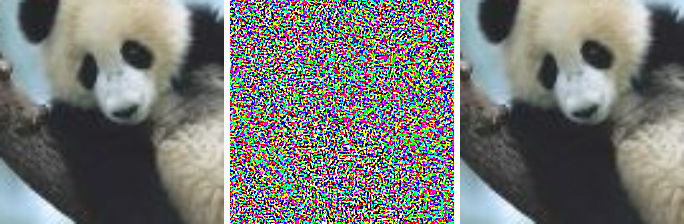
\includegraphics[width=\textwidth]{images/harnessing_ae.png}
	\caption{Original image (left) and adversarial example (right, classified as \emph{gibbon} with $99.3\%$ confidence) with magnified perturbation in the middle, as presented in \cite{explaining-and-harnessing-adversarial-examples}}
	\label{fig:harnessing-ae}
\end{figure}

Of course, linearization of the loss function (which includes the entire network) around $x$ is a rather strong assumption\footnote{Below we will discuss a linear explanation for the existence of adversarial examples, but it does not easily translate to a one-step ae generation algorithm that relies on linearity of the \emph{entire} network}. Rather than making one big leap in the input space, one can easily turn this approach into an iterative procedure of multiple small steps, in the manner of a proper gradient descent. This way, one is able to find nearby AEs even if the linearity assumption is inapplicable, or gives a poor approximation.

% TODO describe iterative algorithm

Even though the FGSM is considerably more efficient compared to the L-BGFS method, repeatedly executing it over numerous iterations again poses the challenge of computation time. At this point it is crucial to realize that the gradient $\nabla_x J$ can be computed efficiently with backpropagation, just like the gradient w.r.t $\theta$. Conceptually, the input can be considered to be just another layer positioned below the first layer of an ANN, merely necessitating another application of the chain rule\footnote{Most neural network software by default won't compute the gradient for the input because it is usually unnecessary. Caffe provides a flag to trigger this computation}. For maximum efficiency, one could even try to integrate AE generation into regular backprop training, with the (possibly minor) complication that AE generation with multiple iterations would be performed in relation to a network with changing weights\footnote{this was not tested in this thesis}.

\subsection{Linear explanation of Adversarial Examples}
\label{subsec:ae-linear-explanation}
% TODO source for resistance against distortions and noise
The existence of adversarial examples naturally begs the question how they are even possible and what parts of a model they can be attributed to. They are a surprise since strict splits into training and test sets were believed to vouch for the generalization abilities of ANNs. Experiments with distorted and noisy input data point in the same direction. Since these methods fail to find significant and systematic flaws in neural networks, it is apparent that adversarial examples reside in narrow, low-probability regions of the data distribution, therefore requiring a directional instead of a randomized search.

% TODO make the linear, high-dimensional explanation a subsection
% TODO better source for linear classifier succeptability to AEs than breaking-linear-classifiers-on-imgagenet
% TODO image from breaking-linear-classifiers-on-imgagenet to show linear classifier AEs
Since AEs hint at precipitous discontinuities in the input-output map realized by the network, it is inviting to blame them on the nonlinear nature of neural networks. However, as pointed out in \cite{breaking-linear-classifiers-on-imgagenet}, even unequivocally linear models such as a softmax linear classifier are succeptable to adversarial examples. An explanation that doesn't require the assumption of neural networks heavily relying on their nonlinear powers was suggested in \cite{explaining-and-harnessing-adversarial-examples}.

This explanation focuses entirely on the linear components of an ANN and high-dimensional input data. Going back to the neuron model layed out in section \ref{sec:artificial-neural-networks}, equations \eqref{eq:neuron-math-membrane-potential} - \eqref{eq:neuron-math-activation-function}, the output of a single unit is computed according to

% TODO better variable names here as well
\begin{align}
	o &= \sigma \braces{\vec{w}^T \vec{i}}
\end{align}

where $\vec{w}$ is the weight vector, $\vec{i}$ an input vector of the same size, $\sigma$ the logistic sigmoid activation function. Lastly, $o$ is the output and the value we want to fudge. Note that $\vec{w}^T \vec{i}$ is simply an inner product, and therefore linear. If the inner product is large, $o$ will approach $1$, and if it reaches very far into the negative range it will approach $0$. Since $\vec{i}$ is the only variable we have control over, this is what we need to use to modify $o$.

% TODO just even $n$, not only powers of 2?
To simplify the scenario, binary vectors $\vec{i}, \vec{w} \in \brackets{0,1}^n$, where $n$ is a power of 2 are considered. This is not a technical necessity and the steps described below would work just the same\footnote{Safe for the coefficient introduced below which would need to scale with the size of the elements of $\vec{i}$}, but it makes for an easily described system. Since the order of the elements of the vectors does not matter, a somewhat orderly weight vector is chosen where the first half contains $+1$ elements and the second half $-1$ elements, so $\vec{w} = \brackets{+1 +1 \dots -1 -1}$. Meanwhile, consider an input of alternating binaries, $\vec{i} = \brackets{+1, -1, +1, -1 \dots}$. In this case, $\vec{w}^T \vec{i} = 0$ holds for symmetry reasons, meaning the neuron is in an undecided state. There is nothing wrong with that, but to fully unfold the effect that is to be demonstrated, the last 4 elements of the input vector are always set to $+1$, leading to $\vec{w}^T \vec{i} = -4$ and subsequently $\sigma \braces{\vec{w}^T \vec{i}} \approx 0.0180$, independently of $n$. This is depicted in figure \ref{fig:ae-explanation} for various powers of $2$ as $n$.

% TODO stack vertically for better readability
\begin{figure}[htp]
    \centering
    \begin{subfigure}[b]{0.45\textwidth}
        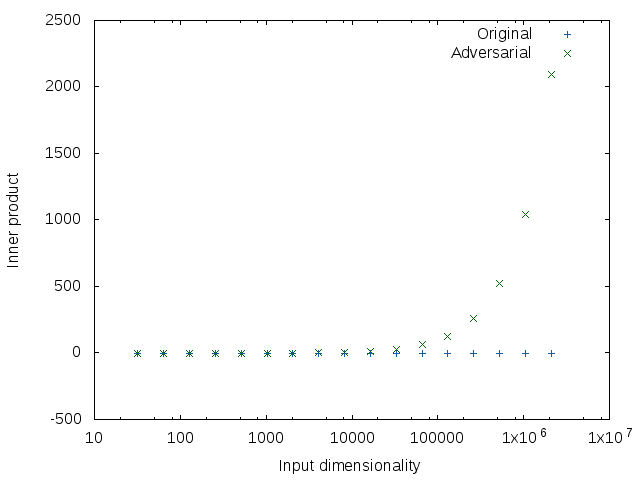
\includegraphics[width=\textwidth]{ae_explanation_ip.png}
        \caption{Inner product of original and adversarial input}
        \label{fig:ae-explanation-inner-product}
    \end{subfigure}
    ~ %add desired spacing between images, e. g. ~, \quad, \qquad, \hfill etc. 
      %(or a blank line to force the subfigure onto a new line)
    \begin{subfigure}[b]{0.45\textwidth}
        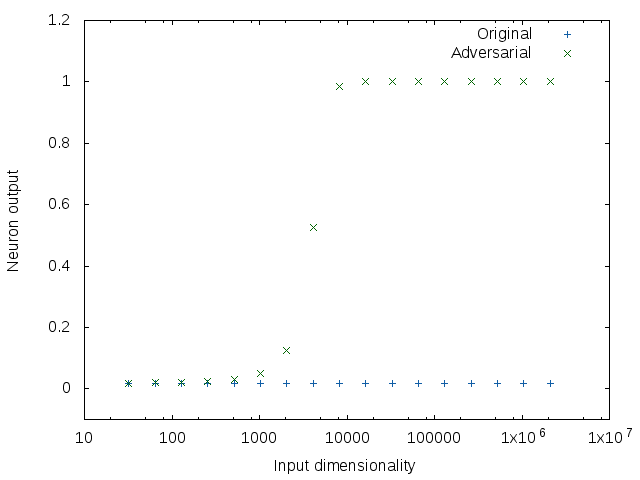
\includegraphics[width=\textwidth]{ae_explanation_output.png}
        \caption{Neuron output for original and adversarial input}
        \label{fig:ae-explanation-neuron-output}
    \end{subfigure}
    \caption{Inner product and neuron output depending in data dimensionality}
    \label{fig:ae-explanation}
\end{figure}

% TODO add a table that shows the same data as the image

For the given input, the neuron is firmly in the off-state. In order to change it to the on-state, the inner product needs to be increased and move into the positive region. Simply put, the inner product will be positive when the input is positive where the weight vector is positive, and negative where the weight vector is negative. Indeed, one could simply set $\vec{i} \coloneqq \sign \braces{\vec{w}}$ since this always fulfills the requirement\footnote{The $\sign$ function is only given to sustain the universality of the approach. Since $\vec{w}$ is a binary vector here, it serves no purpose in this specific context.}. However, that is not a helpful approach when trying to create an adversarial example for the input, since $\vec{i}$ might be vastly different from $\sign \braces{\vec{w}}$. But it is a viable option to change $\vec{i}$ slightly so that it becomes more similar to the sign of the weights. This is described by equation \eqref{eq:ae-explanation-formula}.

% TODO maybe use c instead of \epsilon in eq:fast-gradient-sign-method. It should be the same letter and c is much better.
\begin{align}
	\vec{\hat i}&= \vec{i} + c \cdot \sign \braces{\vec{w}} \label{eq:ae-explanation-formula}
\end{align}

% Note that all of this is similar to the FGSM, but only tries to trick one neuron instead of the network output, and therefore operates on the weight vector instead of the gradient. Can be considered a crude variant of FGSM.
Here, $\vec{\hat i}$ denotes an adversarial example and $c$ is a strength modulation coefficient. It is not surprising that it resembles equation \eqref{eq:fast-gradient-sign-method} for the FGSM, since the goals are similar. But while FGSM tries to trick an entire network, this equation merely tries to change the output of a single neuron in order to demonstrate the susceptibility of (partly) linear models to adversarial perturbation. Since it does not need to take into account how the neuron's output is processed in higher layers of the network, it doesn't operate on the gradient but simply on the weight vector.

The effect of this perturbation is also shown in figure \ref{fig:ae-explanation} for a value of $c = 0.001$. As \ref{fig:ae-explanation-inner-product} demonstrates, the strength of the perturbation's effect on the inner product increases with $n$. It is not surprising that a change of constant size to each element amounts to more the larger the vector is, but what is surprising is the strength of this effect. As figure \ref{fig:ae-explanation-neuron-output} indicates, the critical point where the perturbation forces the neuron into the on-state is located around $n = 4096$.

However, when examining both \ref{fig:ae-explanation-inner-product} and \ref{fig:ae-explanation-neuron-output}, one can see that there is a significant visual discrepancy. The critical point around $4096$ is still in a region where the curve for the inner product is still very flat. This gives reason to believe that with a slight increase in data dimensionality, the method can find adversarial examples even for such input data that leads to a much more confident off-state decision (remember that the original inner product was merely $-4$). It is also worth considering just how small of a change $c = 0.001$ implies. Since the vectors are binary, a change of $0.001$ per element means that each element's value gets changed by only $\frac{1}{1000}$ of its scale. This is a trade-off between dimensionality and $c$, larger input allows for a smaller $c$ while smaller input requires a larger $c$.

In conclusion, one does not need to invoke nonlinear properties of neural networks to explain the existence of adversarial examples. Indeed, it is preferable to not do so, since while a neural network is \emph{potentially} nonlinear owing to their activation functions, most of these\footnote{and, in fact all of those shown in figure \ref{fig:activation-functions}} contain a region that at least approximates a linear function. Thus, basing an explanation on nonlinearity makes some additional assumptions about the distribution of a networks membrane potentials. Instead of that, the linear explanation relies only on properties of the inner product and input data dimensionality. It was demonstrated that it becomes easier and easier to tamper with the value of an inner product, and hence with neuron outputs, as the data size grows, while keeping the changes to each individual value in the input minimal.

% TODO finish this section
\subsubsection{Adversarial Examples in Convolutional Neural Networks}
The explanation given in subsection \ref{subsec:ae-linear-explanation} relates adversarial examples mostly with inner products in high-dimensional spaces. But even though convolutional neural networks are just as susceptible to adversarial examples, their first operation on the input data is usually a convolution which typically uses relatively small filters, in the order of $3 \times 3$ to $7 \times 7$. While it is possible to chose a larger coefficient to have a greater leverage on the the value of the inner product, a reflection on the nature of CNNs allows for a different answer.

% TODO finish this
A crucial point is that the explanation given addresses a single neuron, but a convolutional network consists of many layers, each of which contain numerous neurons. Ultimately, the success of an adversarial example depends on manipulating the values in the last layer, not the first. So while it might not be possibly to have a strong impact on individual neurons in the first convolutional layer, small changes at many points there will be aggregated by subsequent layers\footnote{Note that while this explanation does require more than 1 hidden layer, it does not rely on the nonlinearity between them.}. Thus, in a sense, a CNN also realizes high-dimensional inner products, but defers their computation to higher layers.

\subsection{Universality of Adversarial Examples}
% TODO source for MNIST
% TODO figure out what an autoencoder is
In \cite{intriguing-properties-of-neural-networks}, two more concerning properties of adversarial examples were exposed. Both indicate that AEs are notably more universal than one might expect. The first relates to generalization across multiple models. In the publication, 6 diverse models were trained on the \emph{MNIST} data set, comprising 3 linear softmax classifiers, 2 ANNs with hidden layers and 1 autoencoder. Adversarial examples generated for each of these were evaluated on the other models. The results show that the AEs generalized surprisingly well to other models\footnote{The autoencoder was more resistant to foreign AEs, but still notably more prone to being tricked by them than by random noise on the input data.}.

The other observed property is a universality across different training sets. Neural networks with 2 hidden layers were trained on disjoint, equally large portions of the MNIST training set. Analogously to the above, adversarial examples were generated for each ANN and used for testing on the others. Although they did not retain as much of their deceptive power as they did in the cross-model test, the misclassification rate on the same model trained on seperate data is still considerably higher than both the error on the unmodified test set and random noise.

This universality of AEs is not only astounding, but also problematic since it forecloses a simple solution to the problem. If adversarial examples were model specific, a committee of different or differently trained models could be used to increase resistance against AEs by outvoting the affected model.

\subsection{Relating the Linear Explanation to the Network Function}
% TODO elaborate further on the commented out part
% TODO "is still an open question" as far as I'm aware
Since adversarial examples are able to generalize across both different hyperparameters and different training data choices, their existence seems to be more like a fundamental property of the data space than an a noise-like artifact of a specific network, or of the choice of samples from the data distribution. In \cite{explaining-and-harnessing-adversarial-examples} it has already been established that AEs exhibit some directional contiguity. How this ties in with the topology learned by the network is still an open question. One possible perspective on this matter is attained by considering the function represented by an ANN as a homeomorphism, which is at least valid for nonsingular weight matrices. In that case, the network is only able to stretch and deform the input space as shown in figure \ref{fig:network-homeomorphism} before making a decision, but it can't cut sew up the space.

\begin{figure}[htp]
    \centering
    \begin{subfigure}[b]{0.45\textwidth}
        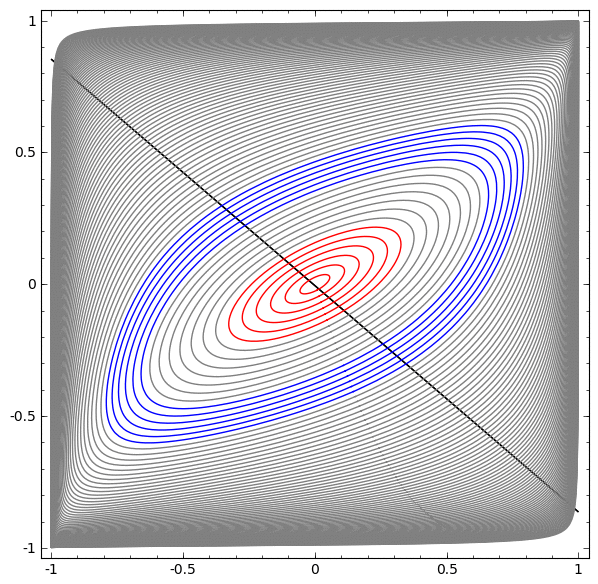
\includegraphics[width=\textwidth]{homeomorphism_start.png}
        \caption{The untransformed input space.}
        \label{fig:network-homeomorphism-start}
    \end{subfigure}
    ~ %add desired spacing between images, e. g. ~, \quad, \qquad, \hfill etc. 
      %(or a blank line to force the subfigure onto a new line)
    \begin{subfigure}[b]{0.45\textwidth}
        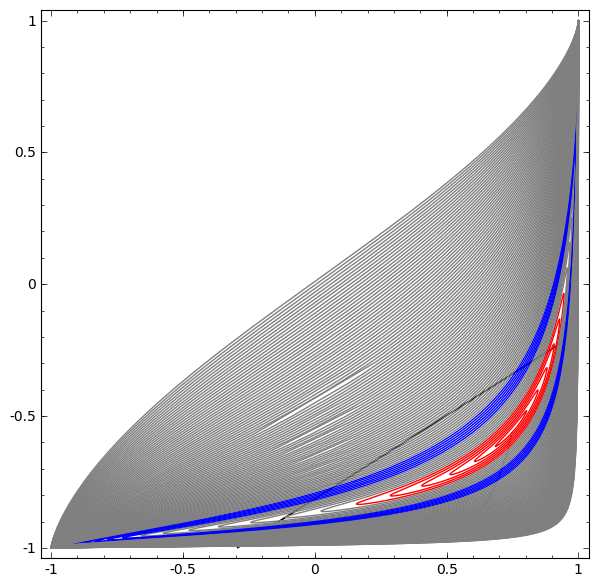
\includegraphics[width=\textwidth]{homeomorphism_end_1.png}
        \caption{Space as transformed by the network.}
        \label{fig:network-homeomorphism-end}
    \end{subfigure}
    \caption{Illustration of a homeomorphic transformation of the input space in a binary classification task Blue and red areas indicate the data distribution and the black line represents the decision boundary. Images taken from \cite{neural-network-homeomorphics-transformation}}
    \label{fig:network-homeomorphism}
\end{figure}

Because the chosen network is not powerful enough to disentangle the classes, it minimizes the average error by elongating the space such that the entangled part becomes minimal. As a consequence the data manifolds for both classes are highly deformed and stretched. A result from \cite{explaining-and-harnessing-adversarial-examples} is that the contiguous regions of adversarial examples radiate outward from the original image. However, since randomized alterations of the input image hardly ever produce adversarial examples, it is clear that if they radiate outwards, they must do so in very thin\footnote{albeit long, and therefore possibly voluminous} strips. The homeomorphic perspective provides a topological reason for the network to do this. Since it can't really \emph{solve} the problem because the data manifolds are too strongly entangled, it minimizes the error by deforming the regions classified erroneously into low probability regions.

% TODO
%% What are they
%% How are they created (two ways)
%% Why is their existence surprising?
%% Deviation from the data manifold?
%% Why do they exist? (strongly fragmented classification regions outside data manifold, lacking smoothness)
%% Linear explanation for AE's existence
%% Generalization across different models and subsets of the data used in training
% They tried to use AEs to train the network to be more resistant, didn't work (but improved generalization)
% Theoretical ramifications for human vision
%% How does the explanation given in "Harnessing AEs" relate to CNNs?
%% Relate existence of AEs with homeomorphism-likeness of ANNs. Harnessing AEs section 8 gives some support
% Points from the summary of Harnessing Adversarial Examples
% How do _I_ create them? The thing with the iterations-dependent coefficient...



% Googlenet
% Describe data sets

\bibliographystyle{alpha}
\bibliography{ref,image-ref}

\end{document}

% List of figures
% List of tables
% List of acronyms

% TODO TODOS
% Be consistent with whether figure captions end with a dot or not.
% Consistent variable names etc.
% Maybe use "dot product" instead of "inner product"?
% Replace can't, don't etc with proper language
% URL in References where important

% Source for CNN performance on image processing tasks
% Alex Krizhevsky, Ilya Sutskever, and Geoff Hinton. Imagenet classification with deep convolutional neural networks. In Advances in Neural Information Processing Systems 25, pages 1106–1114, 2012







